\documentclass{article}

\usepackage[T1]{fontenc}
\usepackage[utf8]{inputenc}
\usepackage{microtype}
\usepackage{graphicx}
\usepackage{booktabs}
\usepackage{longtable}
\usepackage{tabularx}
\usepackage{array}
\usepackage{pdflscape}
\usepackage{xcolor}
\usepackage{enumitem}
\usepackage{listings}
\usepackage[hidelinks]{hyperref}
\usepackage[preprint]{icml2026}

\newcommand{\model}[1]{\textsf{#1}}
\newcommand{\task}[1]{\texttt{#1}}
\newcommand{\pct}[1]{#1\%}
\newcommand{\yes}{\textcolor{green!50!black}{\textbf{pass}}}
\newcommand{\no}{\textcolor{red!65!black}{\textbf{fail}}}
\newcommand{\artifact}{\url{https://github.com/Joey-the-Creater/AlgoVeri-Rerun}}
\newcommand{\lastdance}{\textsc{LastDance}}
\newcolumntype{Y}{>{\raggedright\arraybackslash}X}
\lstset{
  basicstyle=\ttfamily\footnotesize,
  breaklines=true,
  frame=single,
  columns=fullflexible,
  keepspaces=true,
  showstringspaces=false
}

\icmltitlerunning{LastDance: Extending AlgoVeri's Lean Evaluation}

\begin{document}

\twocolumn[
  \icmltitle{\lastdance: Beyond the 7.8\% Lean Baseline with\\
  Frontier Models, Agentic Repair, and Evaluator Audits}

  \begin{icmlauthorlist}
    \icmlauthor{Joey Li}{ind}
  \end{icmlauthorlist}
  \icmlaffiliation{ind}{University of Toronto, Toronto, Canada}
  \icmlcorrespondingauthor{Joey Li}{joeyyizhi.li@mail.utoronto.ca}
  \icmlkeywords{verified code generation, Lean, coding agents, benchmark evaluation,
  LLM-as-a-judge, ICML}
  \vskip 0.3in
]

\printAffiliationsAndNotice{}

\begin{abstract}
AlgoVeri established a challenging baseline for verified code generation on 77 aligned
classical algorithms: its strongest reported Lean system achieved 9.1\% compiler
verification and 7.8\% full marks after semantic filtering.  We extend that study along
three axes: newer frontier models, \lastdance---a constrained Claude Code + Opus 5
toolchain---and an audit of the evaluation pipeline.  Complete-output direct conditions
now compile 92.2--98.7\% of
the Lean tasks, but only 31.2--57.1\% receive full marks, depending on generator and
semantic judge.  Thus, the dominant bottleneck shifts from constructing a compiling
Lean artifact to preserving the requested algorithm under an extensional formal
contract.  On a controlled 65-task subset without teacher-provided proof holes, a
\lastdance compiles 63/65 tasks and passes 53/65 under
GPT-5.4 and 55/65 under GPT-5.6-sol at temperature zero, compared with 39/65 and
44/65 for the strongest complete direct condition.  We contextualize these outcomes
against open systems.  The original open-weight end-to-end conditions peak at 14.3\%
full marks, whereas Goedel-Code-Prover-8B reports 62.3\% proof completion on AlgoVeri.
The latter solves a different, proof-only task over GPT-5.2-generated, manually checked
implementations and therefore is complementary rather than directly rank-comparable.
Using AlgoVeri's original seven categories, \lastdance obtains 100\% full marks on
Basic Data Structures and DP/Algo but 54\% on Graph tasks, extending rather than
eliminating the original complexity cliff.  Cumulative compilation rises from 23\% at
the first observed Lean check to 95\% by the fifth, directly exposing the return from
compiler-grounded repair.

These results confirm AlgoVeri's algorithmic-fidelity gap, extend its finding that
frontier systems exploit iterative repair, and revise the characterization of Lean's
barrier: compilation is no longer the principal failure mode for the evaluated
frontier systems, while semantic degeneracy remains pervasive.  We additionally find
that one immutable scaffold is malformed, 12 tasks expose a contradiction between
teacher-permitted \texttt{sorry} and the judge policy, and two temperature-zero judges
disagree on 22/334 compiled condition--task pairs.  We release all generations,
judge views, case-level analyses, an agent harness, and an interactive audit dashboard.
Our evidence motivates a multi-axis protocol that reports output coverage, formal
verification, algorithmic fidelity, and evaluator robustness separately.
\end{abstract}

\section{Introduction}

Formal verification offers a stronger correctness signal than unit tests: a verifier
checks a program against a mathematical contract.  Yet a verified program is only as
informative as that contract.  A generated Lean file can type-check while implementing
the wrong algorithm, delegating to a library theorem, invoking a nonconstructive
specification oracle, or retaining an unverified teacher placeholder.  Consequently,
verified code generation must measure both \emph{formal correctness} and
\emph{algorithmic fidelity}.

AlgoVeri introduced an unusually controlled setting for this question: 77 textbook
algorithms with aligned natural-language requirements and functional contracts in
Dafny, Verus, and Lean\cite{zhao2026algoveri}.  The original evaluation established
three findings that motivate this work.  First, vericoding remained far from solved,
with the strongest Lean condition obtaining only 9.09\% compiler verification and
7.79\% full marks.  Second, compiler verification systematically exceeded semantic
acceptance, revealing an algorithmic-fidelity gap.  Third, frontier models converted
iterative verifier feedback into progress, whereas weaker systems saturated early;
Lean failures combined proof search and logical reasoning barriers.

We ask what remains true after substituting newer frontier models and a modern coding
agent into the same Lean task suite.  The answer is not simply that scores increase.
Compilation rises above 92\% for every complete direct condition, yet semantic success
lags by 42--66 percentage points.  The capability frontier has therefore moved across
the compiler boundary without eliminating the benchmark's central fidelity problem.
\lastdance closes much of this gap, but its remaining failures reveal
a stable optimization pressure toward brute-force solvers, classical choice, and
verified fallbacks.  Meanwhile, evaluator defects introduce measurement error precisely
where scores are becoming large enough for reliable ranking to matter.

This paper makes six contributions:

\begin{enumerate}[leftmargin=*,itemsep=2pt]
  \item We extend AlgoVeri's Lean evaluation with four direct frontier-model conditions
        and three semantic-judge conditions, placing every result against the original
        paper's capability, fidelity, and repair findings.
  \item We introduce \lastdance, an isolated Claude Code + Opus 5 toolchain with
        constrained compiler access, adaptive repair, source-ownership enforcement,
        and final independent verification.
  \item We show a bottleneck shift: current frontier models largely overcome Lean
        compilation, while algorithm identity becomes the dominant source of failure.
  \item We compare against both general open-weight end-to-end generators and
        purpose-trained open neural provers, identifying task definition and inference
        budget as essential axes of any AlgoVeri comparison.
  \item We audit every compiler failure, every \lastdance semantic rejection, every
        judge disagreement, and all task-level outcomes.  The complete matrix appears
        in Appendix~\ref{tab:complete-matrix}; machine-readable analyses are released
        with the artifact\cite{rerunrepo}.
  \item We identify a malformed scaffold, an ownership contradiction involving
        teacher-permitted \texttt{sorry}, an asymmetric repair prompt, and measurable
        judge dependence, then propose concrete benchmark fixes.
\end{enumerate}

This is a Lean-only extension, not a reproduction of AlgoVeri's cross-language ranking.
Because model endpoints, inference controls, and semantic judges differ, comparisons to
the original reported rates are descriptive historical comparisons rather than a
causal estimate of model progress.

\section{Background and Related Work}

\subsection{Lean and verified code generation}

Lean 4 combines dependent type theory, an extensible theorem prover, and a functional
programming language\cite{demoura2021lean4}.  Mathlib supplies a large, community-built
library of definitions, theorems, and tactics\cite{mathlib2020}.  This ecosystem enables
machine-checkable proofs but also creates evaluation choices: using Mathlib is necessary
for the supplied tasks, whereas calling an existing implementation of the target
algorithm may violate a ``from scratch'' requirement.  The benchmark therefore needs a
semantic policy in addition to compiler verification.

Formal-reasoning benchmarks such as miniF2F\cite{zheng2022minif2f} and
LeanDojo\cite{yang2023leandojo} primarily evaluate theorem proving.  Verified program
generation additionally requires executable definitions, functional contracts,
termination, and algorithm-specific invariants.  DafnyBench\cite{loughridge2024dafnybench}
and the multi-language vericoding benchmark\cite{bursuc2025vericoding} demonstrate the
growing interest in this broader setting.  AlgoVeri contributes aligned classical
algorithm tasks across verification paradigms\cite{zhao2026algoveri}.

The broader open-mathematics frontier spans increasingly demanding task definitions.
PutnamBench supplies hand-constructed, multilingual formalizations of undergraduate
competition theorems and can separate answer discovery from proof completion
\cite{tsoukalas2024putnambench}.  OpenChallenge-style, evolving collections such as
Formal Conjectures move toward active research mathematics, including open statements
designed to limit contamination~\cite{firsching2026formalconjectures}; the living
Erd\H{o}s Problems catalogue provides another prominent source of long-horizon open
questions~\cite{erdosproblems}.  These settings are not interchangeable with AlgoVeri:
they emphasize mathematical discovery or proof synthesis, whereas AlgoVeri jointly
tests implementation choice, executable code, proof construction, and algorithmic
fidelity.  Nevertheless, their shared need for persistent decomposition, verifier
feedback, provenance, and auditable stopping criteria motivates studying whether an
agent harness such as \lastdance transfers beyond textbook algorithms.

\subsection{AlgoVeri's two-stage Lean metric}

Each Lean task contains a natural-language description and a scaffold with four
model-editable marker regions: \texttt{auxcode}, \texttt{code}, \texttt{lemma}, and
\texttt{proof}.  The response parser copies only those regions into the teacher
scaffold.  Generated uses of \texttt{sorry}, \texttt{admit}, axioms, unsafe definitions,
and related bypasses are rejected.  A local Lean compiler then checks the merged file.

Compilation alone cannot enforce the named algorithm.  AlgoVeri therefore applies an
LLM semantic filter to the natural-language task and complete merged file.  The judge
checks whether the intended algorithm was implemented from scratch and whether the
answer uses a compiler trick.  This is an instance of model-based evaluation, whose
scalability comes with known sensitivity to judge and prompt\cite{zheng2023llmjudge}.
We retain the benchmark prompt while explicitly measuring that sensitivity.

\subsection{Open and open-weight systems}

AlgoVeri's original evaluation includes four general open-weight model families:
GPT-OSS-120B, Qwen3-235B-A22B-Instruct, Qwen3-Next-80B-A3B-Thinking, and
Devstral-2-123B-Instruct\cite{zhao2026algoveri}.  These systems face the full task:
generate the requested implementation and proof, repair compiler errors, and pass the
semantic filter.  They are therefore methodologically close to our direct conditions,
although model versions, sampling multiplicity, and infrastructure differ.

Goedel-Code-Prover takes a different route\cite{li2026goedelcodeprover}.  Its open 8B
policy recursively decomposes a verification theorem, checks candidate lemmas through
proof reconstruction and QuickCheck, and iteratively completes the leaves with Lean
feedback.  On AlgoVeri and CLEVER, however, the implementation is not generated as part
of the reported proving trial: GPT-5.2 first generates code that the authors manually
verify, after which the system synthesizes the remaining proof.  Its baselines include
Kimina-Prover-72B, DeepSeek-Prover-V2-671B, Goedel-Prover-V2-32B, and
BFS-Prover-V2-32B at pass@128.  This proof-only formulation isolates proof search and
cannot measure the algorithmic-fidelity failures central to AlgoVeri's original full-
mark metric.

\section{Extending AlgoVeri's Findings}
\label{sec:extension-framework}

Table~\ref{tab:extension-map} states the relationship between the original conclusions
and our extension.  We treat the published AlgoVeri rates as a historical reference,
retain its compile-then-semantic evaluation logic, and introduce controlled analyses
where the original protocol leaves evaluator uncertainty unmeasured.

\begin{table*}[t]
\centering
\small
\caption{How this study extends the principal findings of AlgoVeri.  Numerical
comparisons across papers are descriptive because models and endpoint controls differ.}
\label{tab:extension-map}
\begin{tabularx}{\textwidth}{>{\raggedright\arraybackslash}p{0.18\textwidth}YY}
\toprule
Original finding & Evidence in this extension & Updated interpretation \\
\midrule
Lean is the hardest target; best full mark is 7.79\%. & Complete direct conditions
compile 92.2--98.7\% and obtain 31.2--57.1\% full marks. & The evaluated frontier has
crossed much of Lean's compilation barrier, but vericoding remains unsolved. \\
Compiler verification overstates algorithmic correctness. & The direct-model
compiler-to-semantic gap is 41.6--66.2 percentage points on full-scope conditions. &
The fidelity gap grows more visible as formal compilation becomes easier. \\
Frontier models benefit from iterative repair; weaker models saturate early. & All
complete direct conditions continue gaining compilation successes after the first
round; the agent moves from 15 to 62 successes by its fifth Lean check. & Tool-mediated
repair remains valuable, but compiler feedback optimizes formal acceptance rather than
algorithm identity. \\
General open models saturate under additional sampling. & Original open-weight
end-to-end systems peak at 14.29\% full marks; the specialized open 8B
Goedel-Code-Prover reports 62.3\% proof-only success on fixed implementations. &
Training and hierarchical decomposition can transform proof search, but proof-only and
end-to-end rates answer different questions. \\
Lean combines search and reasoning barriers. & Final direct compilation failures are
few, while semantic failures use wrong algorithms, oracles, and fallbacks. & The
bottleneck shifts from proof search toward specification alignment and algorithmic
fidelity for newer frontier systems. \\
Expert curation and semantic filtering protect benchmark validity. & We find one
uncompilable scaffold, 12 ownership-confounded tasks, and 22/334 cross-judge flips. &
Task curation must be complemented by executable preflight and evaluator calibration. \\
\bottomrule
\end{tabularx}
\end{table*}

We organize the empirical study around six research questions:

\begin{description}[leftmargin=3.2em,style=nextline]
  \item[RQ1] How far has the Lean capability frontier moved relative to AlgoVeri's
             original 9.09\% verified and 7.79\% full-mark reference point?
  \item[RQ2] Does AlgoVeri's algorithmic-fidelity gap persist after compilation becomes
             common rather than exceptional?
  \item[RQ3] Does \lastdance improve end-to-end semantic
             performance relative to direct API generation?
  \item[RQ4] How stable are semantic conclusions under temperature and judge-model
             changes?
  \item[RQ5] Which task, prompt, and evaluator defects threaten the validity of the
             measured score, and how should the protocol change?
  \item[RQ6] How do general open-weight generators and specialized open proof systems
             compare once task definition and inference budget are made explicit?
\end{description}

\section{Experimental Design}

\subsection{Relationship to the original protocol}

Both studies use the same 77 Lean task identities, natural-language algorithm
requirements, four editable regions, iterative compiler feedback, and a semantic filter
after successful compilation.  The direct conditions retain a maximum of 15 attempts,
matching the original study's main repair depth.  Our extension differs in four ways:
it is Lean-only; it evaluates later proprietary model endpoints; it compiles through a
pinned local Lake environment rather than treating the container runtime as essential;
and it adds an agentic treatment plus three judge configurations.  We therefore compare
the \emph{shape} of the findings and report original numbers as context, but reserve
paired statistical tests for conditions evaluated on the same tasks in this artifact.

\subsection{External open-system comparisons}

We transcribe external comparison values from the published AlgoVeri v2 table and
Goedel-Code-Prover v2 experiment figure and setup\cite{zhao2026algoveri,li2026goedelcodeprover}.
They were not rerun in our environment.  We partition them by task definition:
\emph{end-to-end generation} requires synthesizing both implementation and proof and
then applying AlgoVeri's semantic filter; \emph{proof-only completion} supplies a fixed,
manually checked implementation and measures whether the remaining theorem is proved.
For original open-weight models we report the strongest published $10\times15$ setting
(10 independent passes, each with up to 15 repairs).  For proof-only neural baselines we
report pass@128.  Goedel-Code-Prover instead uses hierarchical search with up to 128
decomposition and 128 completion iterations.  We do not run statistical tests across
these incompatible protocols.

\subsection{Task scopes}

The full scope contains all 77 Lean tasks in the public AlgoVeri repository
\cite{algoverirepo}.  Four direct conditions target the full scope.  The adaptive-
thinking Opus run produced only 49 saved outputs; missing outputs remain failures under
the end-to-end denominator and are also reported conditionally.

The \lastdance experiment uses a deterministic source-aware filter that
excludes the 12 tasks containing teacher-owned \texttt{sorry} outside all four editable
regions.  Its scope is therefore 65 tasks.  We evaluate every generator on this same
65-task set for fair comparisons.  No generation result is selected or discarded based
on its later semantic verdict.

\subsection{Direct generation conditions}

We evaluate \model{GPT-5.5}, \model{GPT-5.6-sol}, and \model{Claude Opus 5} through the
same AlgoVeri chat-and-compiler-revision loop.  Each task receives one independent pass,
up to 15 generation or repair attempts, and compiler error feedback after an invalid
attempt.  The OpenAI conditions use medium reasoning and a 32,768-token maximum output.
Opus is evaluated both with adaptive thinking and with thinking disabled.  Provider-
specific reasoning settings are not assumed to be equivalent.

The initial prompt explains the algorithm requirement and prohibits compiler bypasses.
After a failed attempt, the stock Lean revision prompt asks for a complete standalone
file that addresses the compiler errors.  Section~\ref{sec:prompt-audit} discusses the
semantic information lost in this shorter revision instruction.

\subsection{The \lastdance coding-agent condition}

\lastdance uses Claude Code 2.1.220 with \model{Opus 5}, medium effort, and an isolated
workspace per task.  The agent may read task files, edit only
\texttt{Solution.lean}, and invoke only a constrained \texttt{./check.sh}; network,
Git, package installation, and arbitrary shell commands are blocked.  Candidate content
is copied only from the four editable regions into the original scaffold.  The harness
then rejects prohibited terms and independently recompiles the merged result.

The enhanced protocol provides an initial budget of USD~2.  If independent compilation
fails, one fresh compiler-repair session receives the exact verifier feedback and up to
another USD~2 while preserving the workspace.  The prompt explicitly prohibits
alternative algorithms, specification oracles, brute-force enumeration, sorting as a
substitute, \texttt{Nat.find}, \texttt{Classical.choose}, and \texttt{decide} over the
target property.  It also requires an early Lean check and a final requirement-by-
requirement semantic audit.  The final saved result is always independently checked;
the agent's claim of success is not trusted.  Figure~\ref{fig:lastdance-pipeline}
summarizes this trust boundary and the two feedback paths.

\begin{figure*}[t]
  \centering
  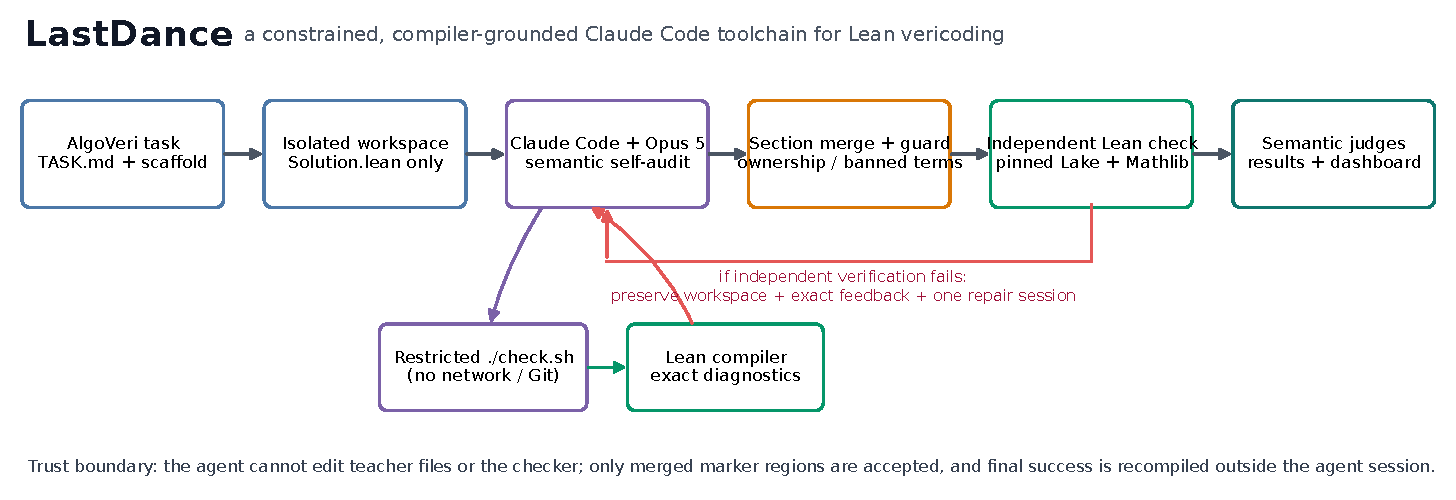
\includegraphics[width=\textwidth]{figures/lastdance_pipeline.pdf}
  \caption{The \lastdance pipeline.  Claude Code can modify only the candidate marker
  regions and interact with Lean through a restricted checker.  Compiler diagnostics
  drive within-session repair.  After marker-aware merging and policy validation, a
  separate Lean invocation rechecks the final candidate; failure can trigger one fresh,
  preserved-workspace repair session.  Semantic judges run only after generation and
  do not guide the reported condition.}
  \label{fig:lastdance-pipeline}
\end{figure*}

Before the final \lastdance run, two targeted pilot batches covered 10 and 20 cases that prior
direct conditions had failed.  Those pilots are reported separately because their
selection and prompt differ from the final 65-task condition.

\subsection{Lean environment}

All candidates are compiled locally without Apptainer.  The runner places a temporary
file inside a pinned Lake project and invokes \texttt{lake env lean}.  The environment
uses Lean 4.25.0-rc2 (commit \texttt{744f9806}), Lake 5.0.0, and Mathlib tag
\texttt{v4.25.0-rc2} (commit \texttt{766e19e7}).  The host runs Ubuntu 22.04.5 LTS on an
AMD Ryzen Threadripper PRO 7985WX (64 physical cores, 128 threads) with 502~GiB RAM.
The visible display adapter is AMD/ATI; generation and semantic inference use remote
APIs, so local GPU performance is not part of the treatment.

\subsection{Semantic judges}

Every saved generation output is evaluated with the same AlgoVeri semantic prompt under
three conditions:

\begin{enumerate}[leftmargin=*,itemsep=2pt]
  \item \model{GPT-5.4}, temperature 1 (the initial rerun configuration);
  \item \model{GPT-5.4}, temperature 0;
  \item \model{GPT-5.6-sol}, temperature 0 and reasoning effort \texttt{none}.
\end{enumerate}

GPT-5.6-sol rejects an explicit temperature when reasoning is enabled in this API, so
\texttt{none} is required to isolate temperature zero.  The temperature-zero outputs
are stored in distinct directories and do not overwrite the initial judgments.  Up to
five turns are allowed only to repair malformed \texttt{<analysis>} and
\texttt{<conclusion>} formatting; this is not a vote across independent samples.

\subsection{Metrics and analysis}

We report four mutually exclusive observable states: missing output, saved output that
does not compile, compiled output rejected by the semantic judge, and compiled output
accepted by the judge.  ``Semantic pass'' always means the conjunction of compiler
success, a parsed judgment, and a \texttt{YES} verdict.  Rates use the stated native or
common scope as denominator; we additionally show output-conditional rates where
missingness is material.

Judge agreement is measured only on compiled outputs evaluated by both judges.  We
report raw agreement and Cohen's $\kappa$\cite{cohen1960kappa}.  Paired agent/direct
comparisons on the same 65 tasks use the exact two-sided McNemar test
\cite{mcnemar1947}; these descriptive $p$-values do not make the fixed task suite a
random population.  Selected binomial intervals are 95\% Wilson intervals
\cite{wilson1927}.  All aggregates are regenerated from JSON by
\texttt{scripts/analyze\_rerun\_results.py}; no table was transcribed from terminal
logs.

\section{Results: From Proof Search to Fidelity}

\subsection{The Lean capability frontier has moved}

\begin{table*}[t]
\centering
\small
\caption{Native-scope results.  Semantic columns show pass counts for GPT-5.4 at
temperature 1 (5.4-T1), GPT-5.4 at temperature 0 (5.4-T0), and GPT-5.6-sol at
temperature 0 (5.6-T0).  Percentages use the native scope, not only returned outputs.}
\label{tab:native-results}
\begin{tabular}{lrrrrr}
\toprule
Generation condition & Output & Lean compile & 5.4-T1 & 5.4-T0 & 5.6-T0 \\
\midrule
GPT-5.5 & 77/77 & 75/77 (97.4\%) & 24/77 (31.2\%) & 24/77 (31.2\%) & 24/77 (31.2\%) \\
GPT-5.6-sol & 77/77 & 71/77 (92.2\%) & 25/77 (32.5\%) & 27/77 (35.1\%) & 30/77 (39.0\%) \\
Opus 5, thinking & 49/77 & 49/77 (63.6\%) & 29/77 (37.7\%) & 29/77 (37.7\%) & 31/77 (40.3\%) \\
Opus 5, no thinking & 77/77 & 76/77 (98.7\%) & 36/77 (46.8\%) & 39/77 (50.6\%) & 44/77 (57.1\%) \\
\lastdance & 65/65 & 63/65 (96.9\%) & 53/65 (81.5\%) & 53/65 (81.5\%) & 55/65 (84.6\%) \\
\bottomrule
\end{tabular}
\end{table*}

Table~\ref{tab:native-results} answers RQ1.  AlgoVeri's strongest original Lean result
was Gemini-3 Flash at 7/77 compiler-verified and 6/77 full-mark tasks
(9.09\% and 7.79\%)\cite{zhao2026algoveri}.  In our later evaluation, when an answer is
returned, compilation is high: GPT-5.5 compiles 75/77
(\pct{97.4}; Wilson 95\% CI [\pct{91.0}, \pct{99.3}]), GPT-5.6-sol 71/77
(\pct{92.2}), and no-thinking Opus 76/77 (\pct{98.7}).  The protocols are not identical,
so these numbers do not isolate model improvement; they nevertheless show that the
observed failure regime has changed.  All 49 saved adaptive-thinking
Opus outputs compile, but 28 tasks have no output, reducing end-to-end compilation to
\pct{63.6}.  In its final one-attempt sweep over the missing set, 24 requests exhausted
32,768 output tokens with thinking blocks only and four ended in provider overload.

Disabling Opus thinking eliminates this coverage failure and is not offset by worse
quality on the matched 49 returned tasks.  On those tasks, thinking versus no-thinking
semantic passes are 29 versus 30 (5.4-T1), 29 versus 31 (5.4-T0), and 31 versus 35
(5.6-T0).  Thus this run provides no evidence that adaptive thinking improves the
matched outcome, while it substantially reduces completion reliability.

\subsection{The fidelity gap widens after compilation}

The central result for RQ2 is the size of the compilation--semantic gap.  AlgoVeri
introduced this gap as evidence that formal verification alone does not guarantee the
requested algorithm.  Our extension shows that the issue becomes more pronounced, not
less, once models compile reliably.  For example,
GPT-5.5 compiles 75 tasks but all three judges accept only 24.  No-thinking Opus compiles
76, while acceptance ranges from 36 to 44.  Even conditional on compilation, GPT-5.4 at
temperature zero accepts 32.0\% of GPT-5.5, 38.0\% of GPT-5.6-sol, and 51.3\% of
no-thinking Opus outputs.  The compiler verifies the submitted theorem; it does not
establish that the program realizes the natural-language algorithm.

The 65-task scope removes the known teacher-\texttt{sorry} confound and makes all final
conditions directly comparable (Table~\ref{tab:common-results}).  GPT-5.5 compiles all
65 yet passes only 24.  No-thinking Opus is the strongest direct condition at 39/65
under 5.4-T0 and 44/65 under 5.6-T0.

\begin{table*}[t]
\centering
\small
\caption{Common 65-task scope with no teacher-owned \texttt{sorry}.  This table should
be used for comparisons with \lastdance.}
\label{tab:common-results}
\begin{tabular}{lrrrrr}
\toprule
Generation condition & Output & Lean compile & 5.4-T1 & 5.4-T0 & 5.6-T0 \\
\midrule
GPT-5.5 & 65 & 65 & 24 (36.9\%) & 24 (36.9\%) & 24 (36.9\%) \\
GPT-5.6-sol & 65 & 60 & 25 (38.5\%) & 27 (41.5\%) & 29 (44.6\%) \\
Opus 5, thinking & 47 & 47 & 29 (44.6\%) & 29 (44.6\%) & 31 (47.7\%) \\
Opus 5, no thinking & 65 & 65 & 36 (55.4\%) & 39 (60.0\%) & 44 (67.7\%) \\
\lastdance & 65 & 63 & 53 (81.5\%) & 53 (81.5\%) & 55 (84.6\%) \\
\bottomrule
\end{tabular}
\end{table*}

\begin{figure*}[t]
  \centering
  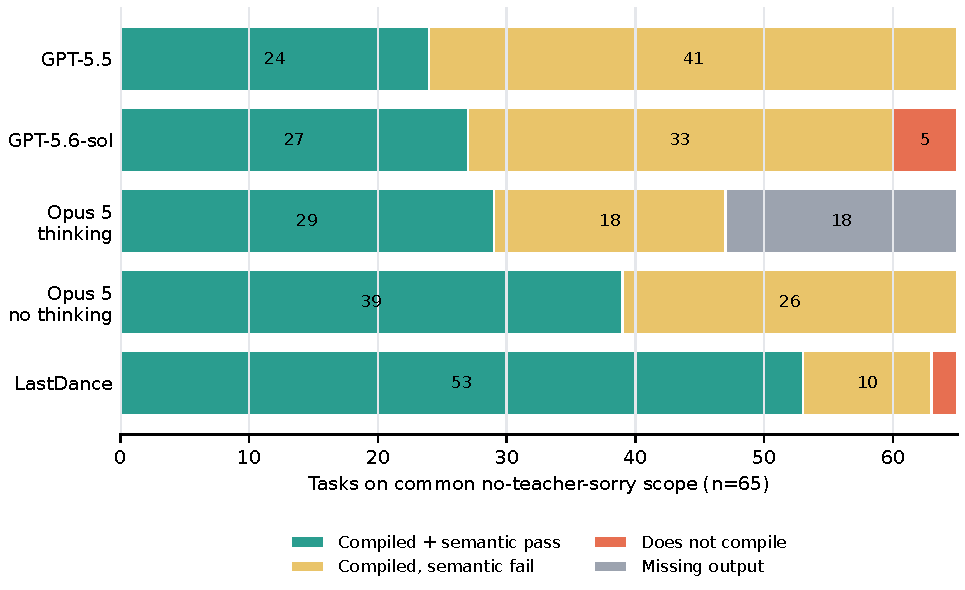
\includegraphics[width=0.76\textwidth]{figures/outcome_breakdown.pdf}
  \caption{Four-state outcome decomposition on the common 65-task scope under the
  GPT-5.4 temperature-zero semantic judge.  Compilation alone hides a large fidelity
  gap for every direct condition.  Missing adaptive-thinking outputs are retained as
  failures; no result is silently dropped.}
  \label{fig:outcome-breakdown}
\end{figure*}

\subsection{\lastdance gains}

\lastdance answers RQ3.  It compiles 63/65 and passes 53/65 under both
GPT-5.4 conditions and 55/65 under GPT-5.6-sol.  Its 5.6-T0 semantic rate is \pct{84.6}
(Wilson 95\% CI [\pct{73.9}, \pct{91.4}]), versus \pct{67.7}
([\pct{55.6}, \pct{77.8}]) for no-thinking Opus on the same tasks.  The agent has 13
unique passes against two unique passes for no-thinking Opus under 5.6-T0 (exact
McNemar $p=0.0074$).  The corresponding discordances are 18--1 under 5.4-T1
($p=7.6\times10^{-5}$) and 16--2 under 5.4-T0 ($p=0.0013$).

This is an agentic condition, not a like-for-like model replacement.  \lastdance receives tool
access, multiple turns, persistent files, explicit semantic reminders, and an adaptive
budget.  The observed gain therefore estimates the whole harness treatment.  The final
65-task run costs USD~70.26 in recorded Claude Code charges (mean USD~1.08 per task) and
contains 6.24 summed agent-hours; direct API dollar cost and duration were not recorded
and cannot be compared.

The earlier targeted pilots compiled 4/10 and 13/20, respectively; combined, 17/30
compiled and 14/30 passed the 5.4-T1 judge at a recorded cost of USD~41.48.  After adding
early checks, a semantic self-audit, a preserved-workspace repair pass, exact verifier
feedback, and final independent verification, the broader \lastdance condition reaches
63/65 compilation and 53/65 5.4-T1 semantic success.  Because task selection and several
settings changed, this is an engineering progression rather than an ablation.

\subsection{Performance by algorithm category}
\label{sec:category-breakdown}

Figure~\ref{fig:category-breakdown} reproduces the seven-way organization used in
AlgoVeri's original category radar plot: Basic Data Structures, Advanced Data
Structures, Sorting, DP \& Algo, Graph, Math, and String\cite{zhao2026algoveri}.  The
original category sizes are 15, 16, 7, 10, 13, 11, and 5 tasks.  Because the controlled
comparison removes teacher-owned \texttt{sorry}, the corresponding common-scope sizes
are 12, 7, 7, 10, 13, 11, and 5.  We report GPT-5.4 temperature-zero full marks so the
generator varies while task scope and judge remain fixed.

\begin{figure*}[t]
  \centering
  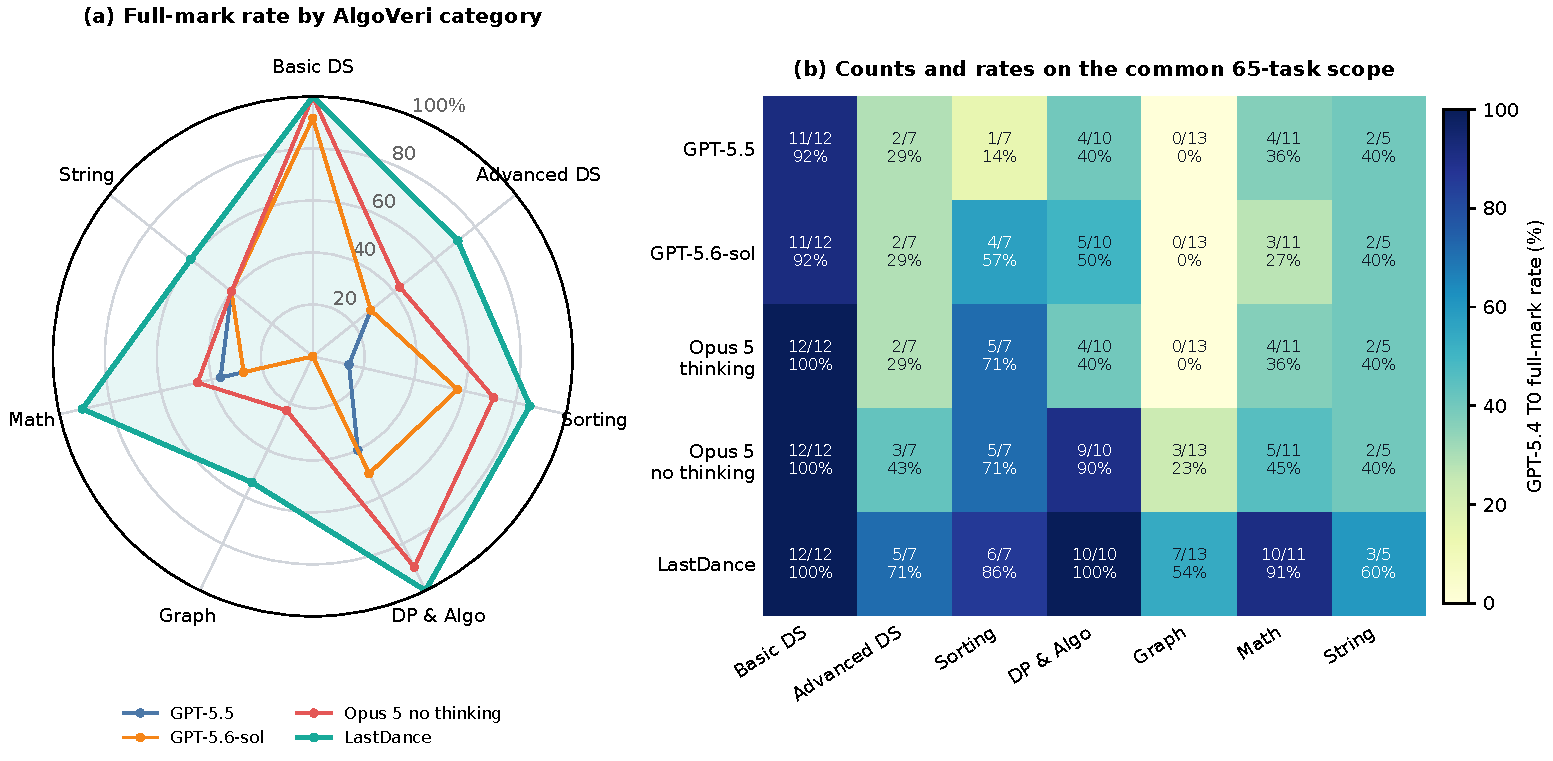
\includegraphics[width=\textwidth]{figures/category_breakdown.pdf}
  \caption{Performance breakdown by the original AlgoVeri algorithm categories on the
  common 65-task scope.  Panel (a) mirrors the original radar presentation for the four
  complete-output conditions; panel (b) shows exact counts and includes
  adaptive-thinking Opus, whose missing outputs remain in each denominator.  Full mark
  denotes compilation plus acceptance by GPT-5.4 at temperature zero.}
  \label{fig:category-breakdown}
\end{figure*}

The original complexity cliff persists but shifts upward.  Basic Data Structures are
nearly saturated: GPT-5.5 and GPT-5.6-sol each pass 11/12, while both Opus variants
and \lastdance pass 12/12.  \lastdance also passes all 10 DP/Algo tasks,
10/11 Math tasks, 6/7 Sorting tasks, and 5/7 controlled Advanced Data Structure tasks.
Graph remains the clearest frontier: GPT-5.5, GPT-5.6-sol, and returned thinking-Opus
answers pass 0/13; no-thinking Opus reaches 3/13, and \lastdance reaches 7/13.  String
tasks remain mixed at 3/5 for \lastdance.  Thus agentic compiler interaction narrows the
category gap without eliminating the global-invariant difficulty highlighted by the
original paper.

\subsection{Open-system comparison}
\label{sec:open-comparison}

Table~\ref{tab:open-comparison} answers RQ6 by separating two evaluation regimes.
Panel~A contains the strongest published settings for AlgoVeri's general open-weight
models.  These are the closest external comparison because they generate implementation
and proof and then face the semantic filter.  GPT-OSS-120B is strongest at 25.97\%
compiler verification and 14.29\% full marks under $10\times15$ sampling.  The Qwen and
Devstral conditions remain below 7\% full marks.  Although not a controlled temporal
comparison, these results place the 31.2--57.1\% full-scope direct rates in this study
well above the original general open-weight frontier.

\begin{table*}[t]
\centering
\small
\caption{Published open/open-weight AlgoVeri comparisons.  Panel A evaluates the
original end-to-end task.  Panel B supplies GPT-5.2-generated, manually checked
implementations and evaluates proof completion only.  ``Full mark'' is therefore not
available for Panel B.  Values are transcribed from the respective papers.}
\label{tab:open-comparison}
\begin{tabular}{llrrr}
\toprule
System & Published protocol & Parameters & Lean verified/proved & Full mark \\
\midrule
\multicolumn{5}{l}{\emph{A. End-to-end implementation + proof + semantic filter (AlgoVeri)}} \\
GPT-OSS & $10\times15$ & 120B & 25.97\% & 14.29\% \\
Qwen3-235B-A22B-Instruct & $10\times15$ & 235B / 22B active & 6.49\% & 6.49\% \\
Qwen3-Next-80B-A3B-Thinking & $10\times15$ & 80B / 3B active & 5.19\% & 5.19\% \\
Devstral-2-Instruct & $10\times15$ & 123B & 6.49\% & 6.49\% \\
\midrule
\multicolumn{5}{l}{\emph{B. Proof-only completion over fixed, manually checked implementations (Goedel-Code-Prover)}} \\
Kimina-Prover & pass@128 & 72B & 15/77 (19.5\%) & n/a \\
DeepSeek-Prover-V2 & pass@128 & 671B & 18/77 (23.4\%) & n/a \\
Goedel-Prover-V2 & pass@128 & 32B & 17/77 (22.1\%) & n/a \\
BFS-Prover-V2 & pass@128 & 32B & 16/77 (20.8\%) & n/a \\
Goedel-Code-Prover & hierarchical search & 8B & 48/77 (62.3\%) & n/a \\
\bottomrule
\end{tabular}
\end{table*}

Goedel-Code-Prover's 48/77 is a strong result for \emph{proof synthesis}: an 8B
domain-trained policy with hierarchical decomposition substantially exceeds much larger
open neural provers\cite{li2026goedelcodeprover}.  It should not be read as 62.3\%
AlgoVeri full marks.  The implementation has already been generated by GPT-5.2 and
manually checked, proof search uses a much larger iterative budget, and no AlgoVeri
semantic-judge score is reported.  Conversely, our conditions must choose the algorithm,
write its implementation, and prove it; their dominant failures often occur in the
first two steps.  The results are thus complementary: Goedel-Code-Prover demonstrates
that explicit lemma decomposition can address the proof-search barrier once a suitable
implementation is fixed, while our study shows that end-to-end agents still need
machine-checkable controls for algorithm identity.

\subsection{Frontier repair remains effective but misaligned}

\begin{figure*}[t]
  \centering
  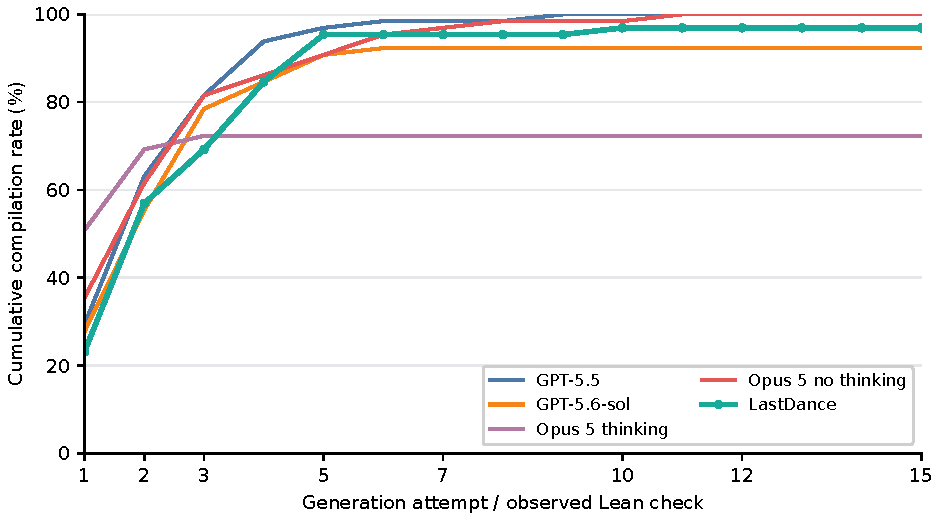
\includegraphics[width=0.76\textwidth]{figures/repair_curves.pdf}
  \caption{Cumulative Lean verification pass rate versus repair depth on the common
  65-task scope.  Direct runs count generation attempts; \lastdance counts observed
  \texttt{./check.sh} invocations.  The horizontal axis therefore measures interaction
  depth, not equal tokens or dollars, and the curves are not pass@$k$ over independent
  samples.}
  \label{fig:repair-curves}
\end{figure*}

Figure~\ref{fig:repair-curves} directly demonstrates the return from compiler feedback.
At the first attempt/check, GPT-5.5, GPT-5.6-sol, no-thinking Opus, and \lastdance verify
19/65, 18/65, 23/65, and 15/65 tasks, respectively.  By depth five those counts reach
63, 59, 59, and 62.  At depth 15 they reach 65, 60, 65, and 63.  Thinking Opus begins
at 33/65 and plateaus at 47/65 by its third attempt because 18 common-scope tasks never
return an output.  The semantic judge was applied only to final candidates, so this
artifact supports a per-round \emph{verification} curve, not a retrospectively inferred
per-round semantic curve.

This pattern extends AlgoVeri's distinction between frontier repair and early
saturation.  The evaluated frontier systems continue converting Lean feedback into
compilation gains, and the \lastdance workspace makes that feedback operationally
effective.  However, compiler feedback contains no signal about whether a different
algorithm or guarded fallback violates the natural-language request.  Repair is thus
effective for the formal objective while remaining partially misaligned with the full-
mark objective.

\subsection{Judge robustness}

Table~\ref{tab:judge-agreement-summary} answers RQ4.  Temperature zero does not
eliminate evaluator variation.  Across all five generation conditions, GPT-5.4 at
temperatures 1 and 0 flips 13 of 334 compiled pairs.  The two temperature-zero judges
flip 22 pairs.  GPT-5.6-sol is more permissive in aggregate: 17 GPT-5.6-only passes
versus five GPT-5.4-only passes, a net gain of 12.

\begin{table*}[t]
\centering
\small
\caption{Pooled semantic-judge agreement on compiled outputs.  A generation of the
same benchmark task is a separate pair; pooled observations are not assumed independent.}
\label{tab:judge-agreement-summary}
\begin{tabular}{lrrrrrr}
\toprule
Comparison & $n$ & Agree & Rate & $\kappa$ & Left only & Right only \\
\midrule
5.4-T1 vs 5.4-T0 & 334 & 321 & 96.1\% & 0.922 & 4 & 9 \\
5.4-T0 vs 5.6-T0 & 334 & 312 & 93.4\% & 0.868 & 5 & 17 \\
\bottomrule
\end{tabular}
\end{table*}

Per-condition agreement ranges from \pct{90.1} to \pct{96.8} for the two zero-
temperature judges.  Exact disagreement cases and directional flips appear in
Appendix~\ref{tab:all-disagreements}.  Several are substantively ambiguous.  For
example, the agent's \task{bubble\_sort} is accepted at 5.4-T1, rejected at 5.4-T0 as
selection-sort-like, and accepted at 5.6-T0.  Its \task{polymul\_naive} is rejected by
GPT-5.4 for an unused placeholder definition but accepted by GPT-5.6-sol based on the
actual convolution implementation.  A single uncalibrated LLM judge should therefore
not be treated as ground truth.

\subsection{Task-level difficulty}

Sixteen tasks are stable successes across every generation condition, every available
output, and all three judges:
\task{bracket\_matching}, \task{bst\_insert}, \task{bst\_search}, \task{bst\_zig},
\task{bst\_zigzag}, \task{bst\_zigzig}, \task{integer\_exponential},
\task{knapsack\_01}, \task{llrbt\_flipcolor}, \task{llrbt\_rotateleft},
\task{matrix\_multiplication}, \task{queue\_dequeue}, \task{queue\_enqueue},
\task{ringbuffer\_enqueue}, \task{stack\_pop}, and \task{stack\_push}.

At the other extreme, under 5.6-T0 no condition passes eight of the 65 controlled tasks:
\task{ac\_automata}, \task{dijkstra}, \task{edmond\_karp}, \task{kruskal},
\task{llrbt\_delete}, \task{longest\_palindrome\_substring}, \task{push\_relabel}, and
\task{scc\_tarjan}.  These concentrate graph invariants, balanced-tree preservation,
and algorithm-identity requirements that are easy to replace with extensional
specification solvers.

\section{Failure Analysis}

\subsection{Compilation failures}

The small number of final compilation failures fall into four distinct classes.

\begin{enumerate}[leftmargin=*,itemsep=3pt]
  \item \textbf{Malformed immutable scaffold.}  \task{trie\_search} fails identically
        for GPT-5.5, GPT-5.6-sol, and no-thinking Opus because the teacher file itself
        contains a duplicate declaration and undefined identifier
        (Section~\ref{sec:trie-defect}).
  \item \textbf{Response-schema failure.}  GPT-5.6-sol's final
        \task{bellman\_ford}, \task{kruskal}, and \task{llrbt\_delete} responses lack
        the required code/proof marker sections.  The parser therefore has no candidate
        to compile.
  \item \textbf{Unresolved Lean proof errors.}  GPT-5.5's \task{trie\_insert} ends with
        tactic and recursion-depth errors.  GPT-5.6-sol's \task{llrbt\_insert} leaves
        type mismatches and unsolved goals, while \task{prim} references an undefined
        helper theorem.
  \item \textbf{Prohibited generated placeholder.}  \lastdance's two failures,
        \task{dijkstra} and \task{kruskal}, reach final candidate validation with an
        editable proof section still containing \texttt{sorry}.  The harness correctly
        records these attempts as failures rather than silently omitting files.
\end{enumerate}

The common compilation problem is therefore not lack of machine resources.  It is a
mixture of benchmark validity, output-protocol compliance, and unfinished proof
construction.  More repair rounds cannot solve immutable scaffolding, and schema-aware
constrained decoding may be more useful than additional proof search for missing marker
regions.

\subsection{Why compiler-accepted programs fail semantically}

Reviewing the judge analyses and generated Lean reveals five recurring patterns.

\paragraph{Different algorithm, correct extensional behavior.}
Many answers prove the supplied input--output property with a simpler algorithm:
insertion or selection behavior for a named sort, direct convolution for Karatsuba,
naive substring search for KMP, mutual reachability for Tarjan SCC, or exhaustive
shortest paths instead of Dijkstra.  Lean correctly verifies the theorem, but the answer
does not satisfy the natural-language algorithm constraint.

\paragraph{Existing verified primitive.}
Examples include computing GCD with \texttt{Nat.gcd} and marking primes with
\texttt{decide (Nat.Prime i)} rather than implementing trial division or a sieve.
These are mathematically valid terms and useful Lean programming patterns, but they
violate the benchmark's from-scratch policy.

\paragraph{Brute force or nonconstructive specification oracle.}
Several answers enumerate all binary vectors for Gaussian elimination, all edge subsets
for matching, or all flow tables for maximum flow.  Others use \texttt{Classical.choose}
or finite search to obtain an object known to satisfy the postcondition.  This behavior
exposes contracts that specify \emph{what} result is correct but cannot encode
\emph{which} algorithm computed it.

\paragraph{Guarded fallback.}
\lastdance often implements a plausible target algorithm but protects it with a
verified reference solver.  The exported function returns the candidate only if a
certificate succeeds; otherwise it rebuilds or brute-forces a correct answer.  Such
fallbacks maximize theorem completion while transferring correctness away from the
named algorithm.

\paragraph{Placeholder or weak helper.}
An unused helper defined as \texttt{0} or \texttt{True}, or a proof that exploits a
weak/vacuous precondition, may compile without providing the intended development.  The
judges differ on whether an unused placeholder alone warrants rejection, contributing
to the disagreement in Section~\ref{tab:judge-agreement-summary}.

\subsection{Residual \lastdance failures}

The two temperature-zero judges agree on eight semantic rejections among the 63 compiled
agent outputs:

\begin{itemize}[leftmargin=*,itemsep=2pt]
  \item \task{ac\_automata}: dynamic suffix search rather than an explicit trie with
        BFS-computed failure links;
  \item \task{edmond\_karp}: a nonconstructive maximum-flow fallback using classical
        choice;
  \item \task{llrbt\_delete}: validate the intended deletion, otherwise rebuild from a
        filtered inorder list;
  \item \task{llrbt\_insert}: flatten, insert into a sorted list, and rebuild instead of
        local LLRBT insertion;
  \item \task{longest\_palindrome\_substring}: guard a Manacher-style candidate with
        exhaustive search;
  \item \task{max\_matching}: enumerate all edge subsets instead of using augmenting
        paths;
  \item \task{push\_relabel}: fall back to exhaustive enumeration of bounded flows;
  \item \task{scc\_tarjan}: compute mutual-reachability classes without Tarjan's stack,
        indices, or low-link values.
\end{itemize}

These failures persist despite explicit prompt prohibitions on exactly these strategies.
Compiler interaction substantially improves theorem completion, but verifier feedback
alone rewards contract satisfaction rather than algorithm identity.  A semantic
self-audit reduces the problem; it cannot provide a machine-checkable enforcement
mechanism.

\section{Evaluation Audit: Extending Quality Control}
\label{sec:benchmark-audit}

AlgoVeri emphasizes expert specification curation and representative formal
well-formedness checks.  Our audit extends that quality-control question from logical
contracts to the executable evaluation pipeline: whether immutable scaffolds compile,
whether authorship is preserved for semantic adjudication, and whether judge decisions
are robust.  RQ5 reveals three independent validity risks.

\subsection{Malformed \task{trie\_search} scaffold}
\label{sec:trie-defect}

The supplied file declares \texttt{is\_valid\_key} twice at lines 59 and 62.  It then
uses an undefined \texttt{well\_formed} at lines 69 and 79.  These locations are outside
all four model-editable sections.  Direct compilation of otherwise different generated
answers consistently reports:

\begin{lstlisting}
line 62: `is_valid_key` has already been declared
line 69: Unknown identifier `well_formed`
line 79: Unknown identifier `well_formed`
\end{lstlisting}

The generation prompt simultaneously requires all non-editable content to remain
unchanged, so no conforming answer can compile.  This is a benchmark defect, not a model
failure.  It lowers end-to-end compilation for every complete full-scope condition by
one and should be repaired or removed before model comparison.

\subsection{Teacher-permitted \texttt{sorry} versus semantic rejection}
\label{sec:sorry-conflict}

The generation prompt expressly warns that some \texttt{sorry} terms occur outside the
editable sections, mostly in \texttt{decreasing\_by} termination proofs, and instructs
the model not to change them.  The response parser likewise checks prohibited terms
only in model-owned regions.  In contrast, the semantic prompt lists visible
\texttt{sorry} as a cheating signal and receives the complete merged file without
machine-readable ownership annotations.

Twelve tasks have teacher-owned \texttt{sorry}: \task{segmenttree\_build},
\task{segmenttree\_modify}, \task{segmenttree\_query}, \task{splaytree\_splay}, the
three ternary-search-tree tasks, the three trie tasks, \task{unionfind\_find}, and
\task{unionfind\_linkroots}.  Across the four direct conditions, 34 returned answers on
this subset compile.  GPT-5.4 assigns zero semantic passes at both temperatures.  Its
analysis of GPT-5.6-sol's \task{ternarysearchtree\_delete}, for example, says the delete
and eager pruning are correct but rejects the answer solely because teacher definitions
contain termination \texttt{sorry}.

GPT-5.6-sol at temperature zero accepts one of the same 34 answers: that exact
\task{ternarysearchtree\_delete}.  Its analysis correctly distinguishes the two
teacher-level termination holes from the student's complete implementation and proof.
This isolated acceptance confirms that ownership-aware adjudication is possible, but
the prompt does not reliably elicit it.  Scores on these 12 tasks conflate student
quality with teacher scaffold policy.

The clean fix is not to allow generated proof holes.  It is to give the judge only the
student-owned sections plus necessary read-only context, or to annotate ownership and
state explicitly that pre-existing teacher holes are permitted.  The enhanced 65-task
condition excludes the confounded tasks instead of retroactively changing their labels.

\subsection{Revision-prompt asymmetry}
\label{sec:prompt-audit}

The initial generation prompt emphasizes the exact natural-language algorithm and
prohibits bypasses.  The subsequent Lean revision prompt says only to correct compiler
messages, provide a complete standalone file, and retain marker structure.  It does not
restate algorithm identity, from-scratch implementation, or the distinction between
teacher and student \texttt{sorry}.  The original system message remains in chat, so
this is an attentional asymmetry rather than a logical permission to cheat.  Nevertheless,
each repair turn makes compiler acceptance the immediate objective, while the later
semantic judge applies the stricter algorithmic criterion.

The observed failures are consistent with this incentive: extensive repairs converge
to classical choice, exhaustive solvers, alternate algorithms, or guarded fallbacks.
\lastdance restates semantic constraints during both initial and repair phases
and performs substantially better, although tool access and budget confound a causal
attribution to prompt design alone.  A controlled ablation is needed to measure the
prompt effect.

\subsection{Metric and reporting implications}

The term ``success rate of Lean'' is ambiguous.  This audit distinguishes at least:
output coverage, parse compliance, compiler verification, absence of prohibited
student terms, algorithmic fidelity, and judge agreement.  A single number hides where
the system failed and can reverse rankings when missing outputs or teacher-owned holes
are handled differently.  We recommend a structured result record rather than a binary
leaderboard field.

\section{Discussion and Recommendations}

\begin{enumerate}[leftmargin=*,itemsep=4pt]
  \item \textbf{Preflight every scaffold.}  Compile a teacher-filled reference after
        erasing only the four student holes; reject duplicate declarations, missing
        identifiers, and version drift before release.
  \item \textbf{Make source ownership explicit.}  Preserve marker provenance through
        semantic evaluation.  Judges should never attribute immutable teacher terms to
        the student.
  \item \textbf{Align all repair prompts.}  Restate the exact-algorithm, from-scratch,
        and no-oracle constraints whenever compiler feedback is supplied.
  \item \textbf{Separate formal and semantic metrics.}  Report output, parse,
        compilation, prohibited-term validation, and semantic fidelity independently.
  \item \textbf{Calibrate semantic evaluation.}  Use temperature-zero runs, at least
        two judges or blinded human adjudication for disagreements, and publish the
        judge model, API mode, prompt, and sampling parameters.
  \item \textbf{Test algorithm identity where possible.}  Add structural obligations,
        trace properties, complexity/resource checks, or required intermediate
        invariants so that a brute-force oracle cannot satisfy the same formal contract.
  \item \textbf{Record every attempt.}  Empty responses, quota errors, overloads,
        parser failures, and prohibited-term candidates should produce durable failure
        artifacts rather than disappearing from the denominator.
  \item \textbf{Evaluate agents as a separate treatment.}  Publish tool policy,
        compiler-call counts, budgets, final independent verification, and costs; do
        not merge agentic scores with direct prompting.
  \item \textbf{Separate proof-only from end-to-end tasks.}  State whether the system
        receives a fixed implementation or must generate it, and never place prove rate
        and semantic full-mark rate in one undifferentiated leaderboard column.
\end{enumerate}

\section{Limitations and Threats to Validity}

\paragraph{Single samples.}
Each generation condition contains one pass per task.  We do not estimate variance over
random seeds, API nondeterminism, or temporal model updates.  Temperature zero is a
sampling setting, not a guarantee of bitwise determinism.

\paragraph{LLM semantic labels.}
No expert manually relabeled all 373 condition--task pairs.  The judge analyses are
useful evidence, not formal proofs of algorithm identity.  The measured 22 cross-judge
flips demonstrate residual label uncertainty.

\paragraph{Unequal treatments.}
Provider reasoning controls and token accounting are not directly comparable.  The
\lastdance receives tools, more interaction, and a monetary budget.  Its result is an
upper-level system comparison, not an isolated Opus model effect.

\paragraph{Externally reported open-system results.}
We did not independently rerun the open/open-weight conditions.  Original AlgoVeri
values use different sampling multiplicities, and the Goedel-Code-Prover comparison
uses fixed manually checked implementations and a substantially larger proof-search
budget.  Its 62.3\% prove rate is neither an end-to-end generation rate nor a semantic
full-mark rate.  The comparison supports qualitative decomposition of capabilities,
not a common-condition ranking.

\paragraph{Adaptive-thinking attrition.}
The 49 returned adaptive-thinking outputs are not a random subset of 77.  Conditional
quality on those outputs is subject to selection bias; end-to-end rates retain missing
outputs in the denominator.

\paragraph{Benchmark and version scope.}
Findings apply to the audited repository snapshot, Lean 4.25.0-rc2, and the named model
endpoints in July--August 2026.  They do not automatically generalize to corrected
scaffolds, other Lean/Mathlib releases, other languages in AlgoVeri, or future endpoint
revisions.

\paragraph{Cost accounting.}
Only \lastdance/Claude Code reports dollar cost in the saved records.  Token fields differ by
provider (for example, Anthropic thinking is not stored in the same field as OpenAI
reasoning), so we release raw counters but avoid a cross-provider efficiency ranking.

\section{Reproducibility and Artifact Layout}

The artifact repository is \artifact.  It includes generation JSON, semantic JSON for
all three judge settings, source modifications, tests, the dashboard, and this report.
The principal immutable directories are:

\begin{itemize}[leftmargin=*]
  \item \texttt{results/full\_three}: GPT-5.5, GPT-5.6-sol, and thinking-Opus generation;
  \item \texttt{results/full\_opus\_no\_thinking}: no-thinking Opus generation;
  \item \texttt{results/claude\_code\_opus5}: enhanced 65-task agent generation;
  \item matching \texttt{\_semantic}, \texttt{\_semantic\_temp0}, and
        \texttt{\_semantic\_gpt56\_temp0} directories for the three judges;
  \item \texttt{reports/data/result\_summary.json} and
        \texttt{reports/data/case\_results.csv}: recomputed aggregate and case-level data;
  \item \path{reports/data/category_results.csv},
        \path{reports/data/repair_curves.csv}, and
        \path{reports/data/outcome_breakdown.csv}: exact values behind the figures;
  \item \path{reports/data/external_open_systems.csv}: published open-system values,
        task definitions, budgets, and comparability annotations;
  \item \path{reports/figures} and \path{reports/prompts}: reproducible vector figures
        and the exact rendered \lastdance prompt templates;
  \item \texttt{config/dashboard\_experiments.json}: the canonical experiment catalog.
\end{itemize}

From the repository root, regenerate the analytical artifacts with:

\begin{lstlisting}
python3 scripts/analyze_rerun_results.py \
  --json-output reports/data/result_summary.json \
  --csv-output reports/data/case_results.csv \
  --latex-output reports/generated/case_tables.tex
python3 scripts/export_lastdance_prompts.py
python3 scripts/generate_report_figures.py
\end{lstlisting}

Compile the paper locally or in Overleaf with:

\begin{lstlisting}
cd reports
latexmk -pdf algoveri_rerun_report.tex
\end{lstlisting}

The CSV contains every judge analysis in full.  The PDF matrix uses compact pass/fail
codes to remain readable; the underlying generated Lean and complete conversations are
preserved in the result JSON.

\section{Conclusion}

AlgoVeri originally showed that Lean vericoding was limited by proof search and
reasoning, that compiler verification exceeded algorithmic correctness, and that
frontier models benefited from repair.  Our extension confirms the latter two findings
while revising the first for current frontier systems.  Complete direct conditions now
compile more than 92\% of tasks, yet attain only 31--57\% full marks.  The principal
bottleneck has shifted from reaching the Lean compiler boundary to preserving the named
algorithm under contracts that admit extensionally correct substitutes.

A constrained coding agent, \lastdance, raises full-mark performance to 82--85\% on the clean
65-task scope, demonstrating that persistent tools and verifier feedback materially
advance the frontier.  Its residual oracle and fallback solutions also show why agentic
compute alone does not solve algorithmic fidelity.  Open-system results sharpen this
decomposition: general open-weight end-to-end models originally peak at 14.3\% full
marks, while Goedel-Code-Prover-8B reaches 62.3\% on the narrower task of proving a
fixed, manually checked implementation.  Specialized hierarchical proof search can
therefore solve much of the proof bottleneck without answering the end-to-end algorithm-
generation question.  Category results preserve AlgoVeri's complexity cliff---Graph
reaches only 7/13 under \lastdance versus 12/12 Basic Data Structures---and the repair
curve shows that most verification gains arrive by the fifth compiler interaction.
Finally, scaffold, ownership, and judge-disagreement findings
extend benchmark quality control beyond specification curation.  Future vericoding
benchmarks should treat implementation synthesis, proof completion, algorithm identity,
provenance, output coverage, and evaluator robustness as distinct measurable objects.

\section*{Impact Statement}

Verified-code agents may reduce the cost of producing high-assurance software, but an
inflated benchmark score can encourage unsafe trust in code that proves the wrong
property or implements the wrong algorithm.  This study's intended impact is improved
measurement: independent compilation, provenance-aware semantic review, and transparent
failure artifacts.  The same techniques could be used to optimize toward benchmark
judges rather than genuine correctness; human review of specifications and disputed
semantic labels therefore remains necessary in safety-critical deployment.

\bibliographystyle{icml2026}
\bibliography{references}

\clearpage
\onecolumn

\appendix

\section{Native-Scope Failure Inventories}

\paragraph{GPT-5.5 compilation failures (2).}
\task{trie\_insert}, \task{trie\_search}.

\paragraph{GPT-5.6-sol compilation failures (6).}
\task{bellman\_ford}, \task{kruskal}, \task{llrbt\_delete}, \task{llrbt\_insert},
\task{prim}, \task{trie\_search}.

\paragraph{No-thinking Opus compilation failures (1).}
\task{trie\_search}.

\paragraph{\lastdance compilation failures (2).}
\task{dijkstra}, \task{kruskal}.

\paragraph{Thinking-Opus missing outputs (28).}
\task{bellman\_ford}, \task{bfs}, \task{coin\_change}, \task{cycle\_detection},
\task{dfs}, \task{dijkstra}, \task{jump\_game}, \task{knapsack\_unbounded},
\task{kruskal}, \task{lca}, \task{llrbt\_delete}, \task{llrbt\_insert},
\task{maxheap\_popmax}, \task{prim}, \task{push\_relabel}, \task{scc\_tarjan},
\task{segmenttree\_modify}, \task{segmenttree\_query},
\task{ternarysearchtree\_delete}, \task{ternarysearchtree\_insert},
\task{ternarysearchtree\_search}, \task{topological\_sort},
\task{trial\_division\_optimized}, \task{trie\_delete}, \task{trie\_insert},
\task{trie\_search}, \task{unionfind\_find}, \task{unionfind\_linkroots}.

\section{\lastdance Prompt Templates}
\label{app:lastdance-prompts}

The following listings are generated directly from the runner functions used for the
reported condition.  \texttt{<TASK\_NAME>} denotes the task-directory name.  The second
listing shows repair pass 2, the only optional fresh repair session in the reported
adaptive configuration; the placeholder between feedback delimiters is replaced by the
verbatim independent verifier response.  Task-specific natural language and the Lean
scaffold are supplied as workspace files rather than interpolated into these prompts.
These are the complete harness-supplied user prompts; Claude Code's vendor-managed
system instructions are external to the repository and are identified indirectly by
the recorded CLI version.

\lstinputlisting[
  caption={Initial \lastdance prompt template.},
  label={lst:lastdance-initial}
]{prompts/lastdance_initial_prompt.txt}

\lstinputlisting[
  caption={Independent-verifier repair prompt template.},
  label={lst:lastdance-repair}
]{prompts/lastdance_repair_prompt.txt}

% Generated by scripts/analyze_rerun_results.py; do not edit manually.
\begin{landscape}
\section{Complete Case Matrix and Judge Disagreements}
\footnotesize
\begin{longtable}{@{}lccccc@{}}
\caption{Complete case-level outcome matrix. A cell is \texttt{C:abc} when Lean compiles; $a$, $b$, and $c$ are semantic outcomes for GPT-5.4 at temperature 1, GPT-5.4 at temperature 0, and GPT-5.6-sol at temperature 0, respectively (\texttt{P}=pass, \texttt{F}=fail). \texttt{X} denotes a saved output that does not compile, \texttt{M} a missing output, and -- an out-of-scope case.}\label{tab:complete-matrix}\\
\toprule
Task & GPT-5.5 & GPT-5.6-sol & Opus think & Opus no-think & Claude Code \\
\midrule
\endfirsthead
\multicolumn{6}{c}{\tablename\ \thetable{} -- continued}\\
\toprule
Task & GPT-5.5 & GPT-5.6-sol & Opus think & Opus no-think & Claude Code \\
\midrule
\endhead
\midrule \multicolumn{6}{r}{Continued on next page}\\
\endfoot
\bottomrule
\endlastfoot
\texttt{ac\_automata} & \texttt{C:FFF} & \texttt{C:FFF} & \texttt{C:FFF} & \texttt{C:FFF} & \texttt{C:FFF} \\
\texttt{bellman\_ford} & \texttt{C:FFF} & \texttt{X} & \texttt{M} & \texttt{C:FPP} & \texttt{C:PPP} \\
\texttt{bfs} & \texttt{C:FFF} & \texttt{C:FFF} & \texttt{M} & \texttt{C:FFF} & \texttt{C:PPP} \\
\texttt{binary\_search} & \texttt{C:FFF} & \texttt{C:PPP} & \texttt{C:PPP} & \texttt{C:PPP} & \texttt{C:PPP} \\
\texttt{bipartite\_check} & \texttt{C:FFF} & \texttt{C:FFP} & \texttt{C:FFP} & \texttt{C:FPP} & \texttt{C:PPP} \\
\texttt{bracket\_matching} & \texttt{C:PPP} & \texttt{C:PPP} & \texttt{C:PPP} & \texttt{C:PPP} & \texttt{C:PPP} \\
\texttt{bst\_delete} & \texttt{C:PPP} & \texttt{C:FFF} & \texttt{C:PPP} & \texttt{C:PPP} & \texttt{C:PPP} \\
\texttt{bst\_insert} & \texttt{C:PPP} & \texttt{C:PPP} & \texttt{C:PPP} & \texttt{C:PPP} & \texttt{C:PPP} \\
\texttt{bst\_search} & \texttt{C:PPP} & \texttt{C:PPP} & \texttt{C:PPP} & \texttt{C:PPP} & \texttt{C:PPP} \\
\texttt{bst\_zig} & \texttt{C:PPP} & \texttt{C:PPP} & \texttt{C:PPP} & \texttt{C:PPP} & \texttt{C:PPP} \\
\texttt{bst\_zigzag} & \texttt{C:PPP} & \texttt{C:PPP} & \texttt{C:PPP} & \texttt{C:PPP} & \texttt{C:PPP} \\
\texttt{bst\_zigzig} & \texttt{C:PPP} & \texttt{C:PPP} & \texttt{C:PPP} & \texttt{C:PPP} & \texttt{C:PPP} \\
\texttt{bubble\_sort} & \texttt{C:FFF} & \texttt{C:FFF} & \texttt{C:PPP} & \texttt{C:PPP} & \texttt{C:PFP} \\
\texttt{coin\_change} & \texttt{C:FFF} & \texttt{C:FFF} & \texttt{M} & \texttt{C:PPP} & \texttt{C:PPP} \\
\texttt{cycle\_detection} & \texttt{C:FFF} & \texttt{C:FFF} & \texttt{M} & \texttt{C:FFP} & \texttt{C:PPP} \\
\texttt{dfs} & \texttt{C:FFF} & \texttt{C:FFF} & \texttt{M} & \texttt{C:FFF} & \texttt{C:PPP} \\
\texttt{dijkstra} & \texttt{C:FFF} & \texttt{C:FFF} & \texttt{M} & \texttt{C:FFF} & \texttt{X} \\
\texttt{discrete\_logarithm} & \texttt{C:FFF} & \texttt{C:PPP} & \texttt{C:FFF} & \texttt{C:PPP} & \texttt{C:PPP} \\
\texttt{edmond\_karp} & \texttt{C:FFF} & \texttt{C:FFF} & \texttt{C:FFF} & \texttt{C:FFF} & \texttt{C:FFF} \\
\texttt{fast\_exponential} & \texttt{C:FFF} & \texttt{C:FFP} & \texttt{C:PPF} & \texttt{C:FFP} & \texttt{C:PPP} \\
\texttt{gcd} & \texttt{C:FFF} & \texttt{C:FFF} & \texttt{C:FFF} & \texttt{C:FFF} & \texttt{C:PPP} \\
\texttt{house\_robber} & \texttt{C:FFF} & \texttt{C:FFF} & \texttt{C:FFF} & \texttt{C:PPP} & \texttt{C:PPP} \\
\texttt{insertion\_sort} & \texttt{C:FFF} & \texttt{C:PPP} & \texttt{C:PPP} & \texttt{C:FFF} & \texttt{C:PPP} \\
\texttt{integer\_exponential} & \texttt{C:PPP} & \texttt{C:PPP} & \texttt{C:PPP} & \texttt{C:PPP} & \texttt{C:PPP} \\
\texttt{jump\_game} & \texttt{C:FFF} & \texttt{C:FFF} & \texttt{M} & \texttt{C:FPP} & \texttt{C:PPP} \\
\texttt{k\_smallest} & \texttt{C:FFF} & \texttt{C:FFF} & \texttt{C:FFF} & \texttt{C:FFF} & \texttt{C:PPP} \\
\texttt{kmp} & \texttt{C:FFF} & \texttt{C:FFF} & \texttt{C:FFF} & \texttt{C:FFF} & \texttt{C:PPP} \\
\texttt{knapsack\_01} & \texttt{C:PPP} & \texttt{C:PPP} & \texttt{C:PPP} & \texttt{C:PPP} & \texttt{C:PPP} \\
\texttt{knapsack\_unbounded} & \texttt{C:PFF} & \texttt{C:FFF} & \texttt{M} & \texttt{C:PPP} & \texttt{C:PPP} \\
\texttt{kruskal} & \texttt{C:FFF} & \texttt{X} & \texttt{M} & \texttt{C:FFF} & \texttt{X} \\
\texttt{lca} & \texttt{C:PFP} & \texttt{C:FPP} & \texttt{M} & \texttt{C:PPP} & \texttt{C:PPP} \\
\texttt{linear\_search} & \texttt{C:PPP} & \texttt{C:PPP} & \texttt{C:FFF} & \texttt{C:PPP} & \texttt{C:PPP} \\
\texttt{linearsys\_gf2} & \texttt{C:FFF} & \texttt{C:FFF} & \texttt{C:FFF} & \texttt{C:FFF} & \texttt{C:PPP} \\
\texttt{llrbt\_delete} & \texttt{C:FFF} & \texttt{X} & \texttt{M} & \texttt{C:FFF} & \texttt{C:FFF} \\
\texttt{llrbt\_flipcolor} & \texttt{C:PPP} & \texttt{C:PPP} & \texttt{C:PPP} & \texttt{C:PPP} & \texttt{C:PPP} \\
\texttt{llrbt\_insert} & \texttt{C:FFF} & \texttt{X} & \texttt{M} & \texttt{C:PPP} & \texttt{C:FFF} \\
\texttt{llrbt\_rotateleft} & \texttt{C:PPP} & \texttt{C:PPP} & \texttt{C:PPP} & \texttt{C:PPP} & \texttt{C:PPP} \\
\texttt{llrbt\_rotateright} & \texttt{C:FFF} & \texttt{C:FFP} & \texttt{C:FFP} & \texttt{C:FFP} & \texttt{C:FPP} \\
\texttt{longest\_common\_subsequence} & \texttt{C:PPP} & \texttt{C:PPP} & \texttt{C:FPP} & \texttt{C:PPP} & \texttt{C:PPP} \\
\texttt{longest\_increasing\_subsequence} & \texttt{C:PPF} & \texttt{C:PPF} & \texttt{C:PPP} & \texttt{C:PPP} & \texttt{C:PPP} \\
\texttt{longest\_palindrome\_substring} & \texttt{C:FFF} & \texttt{C:FFF} & \texttt{C:FFF} & \texttt{C:FFF} & \texttt{C:FFF} \\
\texttt{matrix\_multiplication} & \texttt{C:PPP} & \texttt{C:PPP} & \texttt{C:PPP} & \texttt{C:PPP} & \texttt{C:PPP} \\
\texttt{max\_matching} & \texttt{C:FFF} & \texttt{C:FFF} & \texttt{C:FFP} & \texttt{C:FFP} & \texttt{C:FFF} \\
\texttt{maxheap\_popmax} & \texttt{C:FFF} & \texttt{C:FFF} & \texttt{M} & \texttt{C:FFF} & \texttt{C:PPP} \\
\texttt{maxheap\_push} & \texttt{C:FFF} & \texttt{C:FFF} & \texttt{C:FFF} & \texttt{C:FFF} & \texttt{C:PPP} \\
\texttt{maximum\_subarray\_sum} & \texttt{C:FFF} & \texttt{C:FFF} & \texttt{C:FFF} & \texttt{C:FFF} & \texttt{C:PPP} \\
\texttt{merge\_sort} & \texttt{C:FFF} & \texttt{C:FFF} & \texttt{C:PPP} & \texttt{C:PPP} & \texttt{C:PPP} \\
\texttt{polymul\_karatsuba} & \texttt{C:FFF} & \texttt{C:FFF} & \texttt{C:FFF} & \texttt{C:FFF} & \texttt{C:PPP} \\
\texttt{polymul\_naive} & \texttt{C:PPP} & \texttt{C:FFP} & \texttt{C:PFF} & \texttt{C:FFP} & \texttt{C:FFP} \\
\texttt{prim} & \texttt{C:FFF} & \texttt{X} & \texttt{M} & \texttt{C:FFF} & \texttt{C:PPP} \\
\texttt{push\_relabel} & \texttt{C:FFF} & \texttt{C:FFF} & \texttt{M} & \texttt{C:FFF} & \texttt{C:FFF} \\
\texttt{queue\_dequeue} & \texttt{C:PPP} & \texttt{C:PPP} & \texttt{C:PPP} & \texttt{C:PPP} & \texttt{C:PPP} \\
\texttt{queue\_enqueue} & \texttt{C:PPP} & \texttt{C:PPP} & \texttt{C:PPP} & \texttt{C:PPP} & \texttt{C:PPP} \\
\texttt{quick\_sort} & \texttt{C:FFF} & \texttt{C:PPP} & \texttt{C:PPP} & \texttt{C:PPP} & \texttt{C:PPP} \\
\texttt{ringbuffer\_dequeue} & \texttt{C:FFP} & \texttt{C:FPP} & \texttt{C:PPP} & \texttt{C:PPP} & \texttt{C:PPP} \\
\texttt{ringbuffer\_enqueue} & \texttt{C:PPP} & \texttt{C:PPP} & \texttt{C:PPP} & \texttt{C:PPP} & \texttt{C:PPP} \\
\texttt{rod\_cutting} & \texttt{C:FPF} & \texttt{C:PPP} & \texttt{C:PPP} & \texttt{C:PPP} & \texttt{C:PPP} \\
\texttt{scc\_tarjan} & \texttt{C:FFF} & \texttt{C:FFF} & \texttt{M} & \texttt{C:FFF} & \texttt{C:FFF} \\
\texttt{segmenttree\_build} & \texttt{C:FFF} & \texttt{C:FFF} & \texttt{C:FFF} & \texttt{C:FFF} & -- \\
\texttt{segmenttree\_modify} & \texttt{C:FFF} & \texttt{C:FFF} & \texttt{M} & \texttt{C:FFF} & -- \\
\texttt{segmenttree\_query} & \texttt{C:FFF} & \texttt{C:FFF} & \texttt{M} & \texttt{C:FFF} & -- \\
\texttt{sieve\_method} & \texttt{C:FFF} & \texttt{C:FFF} & \texttt{C:FFF} & \texttt{C:FFF} & \texttt{C:PPP} \\
\texttt{splaytree\_splay} & \texttt{C:FFF} & \texttt{C:FFF} & \texttt{C:FFF} & \texttt{C:FFF} & -- \\
\texttt{stack\_pop} & \texttt{C:PPP} & \texttt{C:PPP} & \texttt{C:PPP} & \texttt{C:PPP} & \texttt{C:PPP} \\
\texttt{stack\_push} & \texttt{C:PPP} & \texttt{C:PPP} & \texttt{C:PPP} & \texttt{C:PPP} & \texttt{C:PPP} \\
\texttt{string\_search\_naive} & \texttt{C:PPP} & \texttt{C:PPF} & \texttt{C:PPP} & \texttt{C:PPP} & \texttt{C:PPP} \\
\texttt{ternarysearchtree\_delete} & \texttt{C:FFF} & \texttt{C:FFP} & \texttt{M} & \texttt{C:FFF} & -- \\
\texttt{ternarysearchtree\_insert} & \texttt{C:FFF} & \texttt{C:FFF} & \texttt{M} & \texttt{C:FFF} & -- \\
\texttt{ternarysearchtree\_search} & \texttt{C:FFF} & \texttt{C:FFF} & \texttt{M} & \texttt{C:FFF} & -- \\
\texttt{topological\_sort} & \texttt{C:FFF} & \texttt{C:FFF} & \texttt{M} & \texttt{C:PPP} & \texttt{C:PPP} \\
\texttt{trial\_division\_naive} & \texttt{C:FPP} & \texttt{C:FFF} & \texttt{C:PPP} & \texttt{C:PPP} & \texttt{C:PPP} \\
\texttt{trial\_division\_optimized} & \texttt{C:FFF} & \texttt{C:FFF} & \texttt{M} & \texttt{C:PPP} & \texttt{C:PPP} \\
\texttt{trie\_delete} & \texttt{C:FFF} & \texttt{C:FFF} & \texttt{M} & \texttt{C:FFF} & -- \\
\texttt{trie\_insert} & \texttt{X} & \texttt{C:FFF} & \texttt{M} & \texttt{C:FFF} & -- \\
\texttt{trie\_search} & \texttt{X} & \texttt{X} & \texttt{M} & \texttt{X} & -- \\
\texttt{unionfind\_find} & \texttt{C:FFF} & \texttt{C:FFF} & \texttt{M} & \texttt{C:FFF} & -- \\
\texttt{unionfind\_linkroots} & \texttt{C:FFF} & \texttt{C:FFF} & \texttt{M} & \texttt{C:FFF} & -- \\
\end{longtable}
\end{landscape}

\begin{landscape}
\subsection{Semantic-Judge Disagreement Inventory}
\scriptsize
\begin{longtable}{@{}llrrrrp{9.2cm}@{}}
\caption{All semantic-judge disagreements on compiler-accepted outputs.}\label{tab:all-disagreements}\\
\toprule
Generation & Comparison & $n$ & Agree & $\kappa$ & Flips & Disagreement cases \\
\midrule
\endfirsthead
\multicolumn{7}{c}{\tablename\ \thetable{} -- continued}\\
\toprule
Generation & Comparison & $n$ & Agree & $\kappa$ & Flips & Disagreement cases \\
\midrule
\endhead
\midrule \multicolumn{7}{r}{Continued on next page}\\
\endfoot
\bottomrule
\endlastfoot
GPT-5.5 & 5.4 T1 vs 5.4 T0 & 75 & 71 & 0.877 & 4 & knapsack\_unbounded (L), lca (L), rod\_cutting (R), trial\_division\_naive (R) \\
GPT-5.5 & 5.4 T0 vs 5.6 T0 & 75 & 71 & 0.877 & 4 & lca (R), longest\_increasing\_subsequence (L), ringbuffer\_dequeue (R), rod\_cutting (L) \\
GPT-5.6-sol & 5.4 T1 vs 5.4 T0 & 71 & 69 & 0.939 & 2 & lca (R), ringbuffer\_dequeue (R) \\
GPT-5.6-sol & 5.4 T0 vs 5.6 T0 & 71 & 64 & 0.795 & 7 & bipartite\_check (R), fast\_exponential (R), llrbt\_rotateright (R), longest\_increasing\_subsequence (L), polymul\_naive (R), string\_search\_naive (L), ternarysearchtree\_delete (R) \\
Opus 5 (thinking) & 5.4 T1 vs 5.4 T0 & 49 & 47 & 0.916 & 2 & longest\_common\_subsequence (R), polymul\_naive (L) \\
Opus 5 (thinking) & 5.4 T0 vs 5.6 T0 & 49 & 45 & 0.828 & 4 & bipartite\_check (R), fast\_exponential (L), llrbt\_rotateright (R), max\_matching (R) \\
Opus 5 (no thinking) & 5.4 T1 vs 5.4 T0 & 76 & 73 & 0.921 & 3 & bellman\_ford (R), bipartite\_check (R), jump\_game (R) \\
Opus 5 (no thinking) & 5.4 T0 vs 5.6 T0 & 76 & 71 & 0.868 & 5 & cycle\_detection (R), fast\_exponential (R), llrbt\_rotateright (R), max\_matching (R), polymul\_naive (R) \\
Claude Code + Opus 5 (enhanced) & 5.4 T1 vs 5.4 T0 & 63 & 61 & 0.881 & 2 & bubble\_sort (L), llrbt\_rotateright (R) \\
Claude Code + Opus 5 (enhanced) & 5.4 T0 vs 5.6 T0 & 63 & 61 & 0.871 & 2 & bubble\_sort (R), polymul\_naive (R) \\
\end{longtable}
\end{landscape}


\end{document}
